\documentclass[11pt, oneside]{article}   	% use "amsart" instead of "article" for AMSLaTeX format
\usepackage{geometry}                		% See geometry.pdf to learn the layout options. There are lots.
\geometry{letterpaper}                   		% ... or a4paper or a5paper or ... 
%\geometry{landscape}                		% Activate for for rotated page geometry
%\usepackage[parfill]{parskip}    		% Activate to begin paragraphs with an empty line rather than an indent
\usepackage{graphicx}				% Use pdf, png, jpg, or eps� with pdflatex; use eps in DVI mode
								% TeX will automatically convert eps --> pdf in pdflatex		
\usepackage{amssymb}

%citation package
\usepackage[square]{natbib}

%package to make contents page with all sorts of tricks
\usepackage{titletoc}

%package for boxes
\usepackage[listings]{tcolorbox}

%maths packages
\usepackage{amsmath}
\usepackage{bm}

%tool for multiple option equations
 \usepackage{mathtools}
 
 %package to allow multi-page table
\usepackage{longtable}

%package for changing depth of table rows
\usepackage{array}

%do more detailed things with the inumerate package
\usepackage{enumerate}

%define vector style
\renewcommand{\vec}[1]{\bm{#1}}

%for using hyperlinks
\usepackage{hyperref}

%allows for code snippets 
\usepackage{listings}
\usepackage{color}

\definecolor{mygreen}{rgb}{0,0.6,0}
\definecolor{mygray}{rgb}{0.5,0.5,0.5}
\definecolor{mymauve}{rgb}{0.58,0,0.82}

\lstset{ %
  backgroundcolor=\color{white},   % choose the background color; you must add \usepackage{color} or \usepackage{xcolor}
  basicstyle=\footnotesize,        % the size of the fonts that are used for the code
  breakatwhitespace=false,         % sets if automatic breaks should only happen at whitespace
  breaklines=true,                 % sets automatic line breaking
  captionpos=b,                    % sets the caption-position to bottom
  commentstyle=\color{mygreen},    % comment style
  deletekeywords={...},            % if you want to delete keywords from the given language
  escapeinside={\%*}{*)},          % if you want to add LaTeX within your code
  extendedchars=true,              % lets you use non-ASCII characters; for 8-bits encodings only, does not work with UTF-8
  frame=single,	                   % adds a frame around the code
  keepspaces=true,                 % keeps spaces in text, useful for keeping indentation of code (possibly needs columns=flexible)
  keywordstyle=\color{blue},       % keyword style
  language=bash,                 % the language of the code
  otherkeywords={*,...},           % if you want to add more keywords to the set
  numbers=left,                    % where to put the line-numbers; possible values are (none, left, right)
  numbersep=5pt,                   % how far the line-numbers are from the code
  numberstyle=\tiny\color{mygray}, % the style that is used for the line-numbers
  rulecolor=\color{black},         % if not set, the frame-color may be changed on line-breaks within not-black text (e.g. comments (green here))
  showspaces=false,                % show spaces everywhere adding particular underscores; it overrides 'showstringspaces'
  showstringspaces=false,          % underline spaces within strings only
  showtabs=false,                  % show tabs within strings adding particular underscores
  stepnumber=1,                    % the step between two line-numbers. If it's 1, each line will be numbered
  stringstyle=\color{mymauve},     % string literal style
  tabsize=2,	                   % sets default tabsize to 2 spaces
  title=\lstname                   % show the filename of files included with \lstinputlisting; also try caption instead of title
}




\title{HERCULES version 1.0 tutorial}
\author{Simon J. Lock}
\date{Last updated:  \today }							% Activate to display a given date or no date

\begin{document}
\maketitle

\makeatletter
\@starttoc{toc}
\makeatother

\clearpage
\clearpage

%%%%%%%%%%%%%%%%%%%%%%%%%%%%%%%%%%%%%%%%%%%%%%%%%%%%%
%%%%%%%%%%%%%%%%%%%%%%%%%%%%%%%%%%%%%%%%%%%%%%%%%%%%%
%%%%%%%%%%%%%%%%%%%%%%%%%%%%%%%%%%%%%%%%%%%%%%%%%%%%%
\section{Introduction}

This tutorial provides an introduction to HERCULES v1.0 and its basic functionality. It is not intended to provide rigorous instruction on using HERCULES and it is recommended that users intending to use HERCULES at more than an introductory level should also read the users manual. 

To complete this tutorial you will need a compiled version of HERCULES and the files that accompany this guide. Consult the users guide for notes on compiling HERCULES. To use the analysis scripts provided with this tutorial you will need to have python installed. To test you have all the libraries required for this tutorial run the script \texttt{test\_python\_libraries.py} that accompanies this tutorial.

%%%%%%%%%%%%%%%%%%%%%%%%%%%%%%%%%%%%%%%%%%%%%%%%%%%%%
\subsection{Overview of HERCULES}

HERCULES - short for Highly Eccentric Rotating Concentric U (potential) Layers Equilibrium Structure - is a code designed to find the equilibrium structure of fluid planets including bodies that are rotating rapidly. The theoretical framework for the code is based on work originally done for studying Jupiter \citep{Hubbard2012, Hubbard2013}  but extended to overcome the problems of numerical convergence in modelling highly oblate bodies \citep{Hubbard2014, Kong2013}.

\begin{figure}[h!]
   \centering
   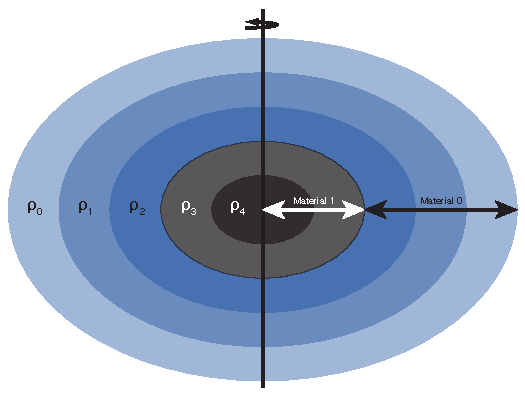
\includegraphics{Figures/HERCULES_schematic.pdf} 
   \caption{Schematic of an axisymmetric, rotationally-flattened planetary structure modelled by the HERCULES code showing a plane through the rotation axis. The modelled body consists of a number of overlapping spheroids, each with constant density, $\delta \rho_i$. The sum of the density of all the individual spheroids overlapping a given layer gives the total density of that layer, $\rho_i$. The body is also divided into a number of material layers (shown separately in blues and greys) with the relationship between pressure and total density in that material layer determined by the material equation of state.}
   \label{fig:schematic}
\end{figure}

In HERCULES, a planet is modelled as a series of concentric constant density layers, made by superimposing constant density spheroids (see box below for notes on terminology and Figure \ref{fig:schematic}).
The gravitational potential due to each of the spheroids can be calculated and summed to give the total potential at a point in the structure as a expansion in spherical harmonics.
Using this useful fact, the shape of each of the spheroids is iterated until the surface of each of the spheroids is an equipotential surface, i.e. to give the equilibrium structure of the planet.
The code can also iterate to conserve the mass of a number of material layers and the total angular momentum of the structure.

The surface of each of the spheroids, and hence layers, is described by a number of points, linearly spaced in $\mu=cos\theta $, where $\theta$ is the angle from the rotation axis.
The material layers (e.g. core, lower mantle, upper mantle etc.) are treated as real materials with equations of state (EOSs) that can be used to give self-consistent densities for each of the concentric layers.  
Spheroids, layers and materials are numbered from the outside in starting from $0$.
A layer is considered as being in a material layer if it's outside surface is within or at the edge of that material layer.

%
\vspace{0.5cm}
\begin{tcolorbox}[colback=white, colframe=red!75!black, title=Note on nomenclature]
In this users guide we use a number of different terms to describe the concentric layers, material layers etc.. 
Here we attempt to clarify the meaning of each of these.

\setlength{\parskip}{15pt}
\setlength{\leftskip}{1.5cm}
\setlength{\parindent}{-1.5cm}
{\it spheroid} or {\it concentric spheroid:} \newline
This refers to the concentric spheroids that make up a planet in HERCULES. 
We use this term to refer to the whole spheroid, which extends from the origin out to the surface of the spheroid.
Each spheroid has a density $\delta \rho_i$.

{\it layer} or {\it concentric layer:} \newline
 A concentric layer is the volume that is bounded by the surfaces of two adjacent spheroids.
The density of a layer, $\rho_i$, is given by the sum of all the spheroids that intersect the layer.
The properties of the layer are the 'real' properties of the planet described by HERCULES.


{\it material layer:} \newline  
A material layer is a compositional or thermal layer in a planet e.g. core, lower mantle, upper mantle etc.
A material layer is the region of the planet that is considered to be of a given material. 
The 'real' density of the layers in this region are calculated using the EOS of that material.
A layer is considered to be part of a given material layer if there outer surface lies within, or at the top of, the material layer.


\setlength{\leftskip}{0pt}
\setlength{\parskip}{0 pt}
\setlength{\parindent}{15pt}

\end{tcolorbox}

%%%%%%%%%%%%%%%%%%%%%%%%%%%%%%%%%%%%%%%%%%%%%%%%%%%%%
%%%%%%%%%%%%%%%%%%%%%%%%%%%%%%%%%%%%%%%%%%%%%%%%%%%%%
%%%%%%%%%%%%%%%%%%%%%%%%%%%%%%%%%%%%%%%%%%%%%%%%%%%%%
\section{Running HERCULES}
\label{sec:running}

To demonstrate how to run HERCULES we will look at a simple example, that of a non-rotating Earth.
This will give us a chance to explore some of the basic options for HERCULES.
In order to run, HERCULES requires an input file called \texttt{HERUCLES\_input.txt} and an output directory \texttt{Output} in the run directory. HERCULES also needs EOS files but the path can be provided for these in the impact directory.

Open the example input file  \texttt{HERCULES\_input\_tutorial1.txt}. You will notice that there are a variety of options in the input file. HERCULES reads in the input file line by line. It is imperative that the format of the file is maintained for correct reading with the option name followed by white space, equals sign, white space and then the variable value. For options that require multiple impacts the options should be given as an array with braces with each element separated by commas. In cases where the inputs are strings leave white space between the strings and commas.

We will now look at some of the options and return to look at the other options later. Leave all the options the same for now.

\setlength{\parskip}{15pt}
\setlength{\leftskip}{1.5cm}
\setlength{\parindent}{-1.5cm}

 {\it run\_name:} The name of the run, or alternatively the name of the body that is being solved for. It is used to name the output files and as an identifier within the output files.

 {\it flag\_Mconc:} The mass conservation flag. There are three options for conserving, or not, the mass of a body. For this tutorial we will only use the option 2, conserving mass by scaling the radius of all of the spheroids. For more detail see the users manual.

 {\it flag\_Lconc:}  The angular momentum conservation flag. There are two possible options: to have a fixed constant rotation rate or conserve angular momentum by adjusting the rotation rate of the body. For now we will use the first of these options.

{\it Nmaterial:} The number of material layers in a body. For now we will just consider two possible layers, mantle and core.

{\it material\_files:} The EOS files for each of the material layers. For this tutorial we will use the precomputed EOS files provided with this tutorial. You will need to make sure that the paths given as input here is correct for where you have put this tutorial relative to your run directory. 

{\it omega\_rot:} The constant angular velocity for the body used for our selected angular momentum conservation flag. \\

\setlength{\leftskip}{0pt}
\setlength{\parskip}{0 pt}
\setlength{\parindent}{15pt} 

Try running HERCULES using the example input file \texttt{HERCULES\_input\_tutorial1.txt} without changing any of the input parameters. You can do this by simply running
\begin{lstlisting}[language=bash]
./HERCULESv1.0 > output.txt
\end{lstlisting}
in the command line. Remember to rename the input file to \texttt{HERUCLES\_input.txt} before running.
If the run is a success then the final line of the output line in the \texttt{output.txt} should read \texttt{run time (s)} followed by a run time. On my 2012 MacBook Pro this example run takes $\sim10$~s. If the run takes significantly longer than this then you might need to check that the paths to the EOS files are correct.

Congratulations, you have made your first planet. In the Output directory you should see two new files. These are HERCULES output files. In the next section we will look at this output.

%%%%%%%%%%%%%%%%%%%%%%%%%%%%%%%%%%%%%%%%%%%%%%%%%%%%%
%%%%%%%%%%%%%%%%%%%%%%%%%%%%%%%%%%%%%%%%%%%%%%%%%%%%%
%%%%%%%%%%%%%%%%%%%%%%%%%%%%%%%%%%%%%%%%%%%%%%%%%%%%%
\section{Understanding the output of HERCULES}

The output for HERCULES comes in two parts, the command line output and binary structure files. We will now look at each of these and explain what they mean. 

%%%%%%%%%%%%%%%%%%%%%%%%%%%%%%%%%%%%%%%%%%%%%%%%%%%%%
\subsection{Command line output}
\label{sec:output}

The command line output is designed to give details about the progress of the code and, in particular, the iterations that are required to find the equilibrium structure. We will break this up to consider each part.

First the start of the file gives information about reading the input file and initialising the structure.

\begin{lstlisting}[language=TeX]
HERCULES is running
Initialising 
	 Reading input file 
	 Run name: tutorial1_L0_N50_Nm400_k6_f020_p10_l1_0_1.5
	 Input file read successful
	 Initialising with ellipsoids
	 	 Using evenly spaced mu points
	 	 Min density 61.962(SI)
	 	 Max density 24786(SI)
	 	 Constant rotation with omega = 0
	 Initialisation complete
\end{lstlisting}

Most of the lines are self explanatory but I will highlight a few.

\setlength{\parskip}{15pt}
\setlength{\leftskip}{1.5cm}
\setlength{\parindent}{-1.5cm}

{\it Line 4:} The name of the file is based on the run name and the properties of the run. For an explanation of this see the users manual.

{\it Line 6:} For this simple example we have used a very simple initialisation routine that initialises the spheroids as each having a constant density. We will look at more options later in \ref{sec:init}. The information in the following indented block gives the resulting maximum and minimum density in the structure and tells us that we are using a constant given rotation rate. \\

\setlength{\leftskip}{0pt}
\setlength{\parskip}{0 pt}
\setlength{\parindent}{15pt}
 
The second section of the file deals with the various iterations used to find the equilibrium structure. 
\begin{lstlisting}[language=TeX]
Iterating
	 Main Iteration # 	 convergence 	 a 	 aspect 	 ellipticity 	 l 	 omega_rot 	 Mass error 	 AM error 
		 Mass/AM Iteration # 	 convergence 	 p_core 	 a 	 omega_rot 	 edge corot 	 AM error 
	 	 	1	1	4.40824e+11	7.84047e+06	0	0	nan
	 	 	2	0.130498	3.89938e+11	6.96949e+06	0	0	nan
	 	 	3	0.0858397	4.26553e+11	6.64456e+06	0	0	nan
	 	 	4	0.00403067	4.2828e+11	6.53605e+06	0	0	nan
	 	 	5	0.0199494	4.19903e+11	6.49422e+06	0	0	nan
	 	 	6	0.0168073	4.12962e+11	6.47517e+06	0	0	nan
	 	 	7	0.0103843	4.08718e+11	6.46527e+06	0	0	nan
	 	 	8	0.00565742	4.06419e+11	6.45968e+06	0	0	nan
	 	 	9	0.00301187	4.05198e+11	6.45705e+06	0	0	nan
	 	 	10	0.00190274	4.04429e+11	6.45588e+06	0	0	nan
	 	 	11	0.00102383	4.04015e+11	6.45518e+06	0	0	nan
	 	 	12	0.000511465	4.03808e+11	6.45475e+06	0	0	nan
	 	 	13	0.000259489	4.03704e+11	6.4545e+06	0	0	nan
	 	 	14	0.000135397	4.03649e+11	6.45436e+06	0	0	nan
	 	 	15	7.25618e-05	4.0362e+11	6.45428e+06	0	0	nan
	 	 	16	3.95117e-05	4.03604e+11	6.45424e+06	0	0	nan
	 	 	17	2.16648e-05	4.03595e+11	6.45422e+06	0	0	nan
	 	 	18	1.1907e-05	4.0359e+11	6.4542e+06	0	0	nan
	 	 	19	6.54797e-06	4.03588e+11	6.4542e+06	0	0	nan
	 	 	20	3.60123e-06	4.03586e+11	6.45419e+06	0	0	nan
	 	 	21	1.98056e-06	4.03585e+11	6.45419e+06	0	0	nan
	 	 	22	1.08922e-06	4.03585e+11	6.45419e+06	0	0	nan
	 	 	23	5.99022e-07	4.03585e+11	6.45419e+06	0	0	nan
	 1	0.310561	6.45419e+06	1	nan	nan	0	4.33676e-07	nan
\end{lstlisting}

HERCULES has a main iteration loop that contains two more separate iterations. The first of the sub-iterations is to find the shape of each of the spheroids but keeps the equatorial radius of each of the spheroids the same. The second iteration changes the equatorial radii and rotation rate of the spheroids to conserve mass and angular momentum. The first of these loops applies to each of the individual points on each of the layers and so is not recorded in the command line output. However, key properties of the structure are given at each iterative step for the conservation and main loops. Line 2 gives the header information for the main loop and Line 27 give an example output for a main iteration. All values are in base SI. The values given are as follows: \\

\setlength{\parskip}{0pt}
\setlength{\leftskip}{1.5cm}
\setlength{\parindent}{-1.5cm}

{\it Iteration \#:} The number of the iteration.

{\it convergence:} The value of the convergence criteria a that iteration.

{\it a:} The equatorial radius of the outermost spheroid.

{\it aspect:} The ratio of the polar radius to the equatorial radius.

{\it ellipticity:} A measure of the flattening of the body. See definition in user manual.

{\it l:} A measure of the flattening of the body. See definition in user manual.

{\it omega\_rot:} The angular velocity of the body.

{\it Mass error:} The fractional difference between the current mass of the body and the target mass.

{\it AM error:} As above but for angular momentum. \\

\setlength{\leftskip}{0pt}
\setlength{\parskip}{0 pt}
\setlength{\parindent}{15pt}

Line 3 gives the header information for the conservation loop and lines 4-26 give the results of a series of iterations for the conservation routine. The values given are some of those given for the main loop with the addition of the folowing \\

\setlength{\parskip}{0pt}
\setlength{\leftskip}{1.5cm}
\setlength{\parindent}{-1.5cm}

{\it p\_core:} Pressure at the centre of the planet.

{\it edge corot:} The layer at the edge of a corotating region. We will not be concerned with this for this tutorial. \\

\setlength{\leftskip}{0pt}
\setlength{\parskip}{0 pt}
\setlength{\parindent}{15pt}

Note that in the example we are using the angular momentum error appears as \texttt{NaN} as the body is non-rotating and so the fractional error in angular momentum is not well defined. 

%%%%%%%%%%%%%%%%%%%%%%%%%%%%%%%%%%%%%%%%%%%%%%%%%%%%%
\subsection{Structure files}

The main output of the code are binary structure files. These contain all the information about a structure and the run that generated it. Here we will describe the structure of the output files and then look at extracting a few of these.

The first part of a structure file holds the information about the run that generated the structure. This is contained in a parameter class object which has the following variables

\clearpage
\begin{longtable}{l l p{10cm}}
\caption{Structure of the parameter class.}
\label{tab:parameters_class} \\
%\vspace{1 cm}

Name & Symbol & Description \\ \hline \hline
\multicolumn{3}{l}{} \\
\endfirsthead

\multicolumn{3}{c}{{\tablename\ \thetable{} -- continued from previous page}} \\
\multicolumn{3}{l}{} \\
\endhead

\multicolumn{3}{l}{} \\
\multicolumn{3}{r}{{continued on next page}} \\
\endfoot

\endlastfoot

\multicolumn{3}{l}{Variables} \\
\hline
\texttt{run\_name} & & Name of the code run (up to 80 characters) \\
\texttt{nint\_max} & $n_{\rm int}$ & Maximum number of iterations for main iteration and mass-AM iteration \\
\texttt{toll} & $\chi_{\rm toll}$ & Desired fractional change in iteration convergence criteria desired for main iteration and mass-AM iteration \\
\texttt{xi\_int\_max} & $n_{\rm int}^{\xi}$ & Maximum number of itterations for shape iteration \\
\texttt{xi\_toll} & $\chi_{\rm toll}^{\xi}$ & Desired fractional change in iteration convergence criteria desired for shape iteration \\
\texttt{dxi} & $\delta \xi$ & $\xi$ step used to calculate the $dU/d\xi$ used in shape iteration \\
\texttt{flag\_start} & $\mathcal{F}_{\rm start}$ & Flag for how to initiate the structure in the code. We will look at this in Section \ref{sec:init} \\
\texttt{start\_file} & & File to use in some initialisation routines. Again we will discuss this in Section \ref{sec:init} \\
\texttt{flag\_Mconc} & $\mathcal{F}_{\rm Mconc}$ & Flag for mass conservation option. For this tutorial, and almost all cases of running HERCULES, we will only use flag 2. \\
\texttt{flag\_Lconc} & $\mathcal{F}_{\rm Lconc}$ & Flag for AM conservation option. We will explore this options in Section \ref{sec:rot} \\
\texttt{flag\_iter\_print} & $\mathcal{F}_{\rm print}$ & Flag for whether to print an output file on every iteration. This will be useful later. \\

\multicolumn{3}{l}{} \\
\multicolumn{3}{l}{Vectors} \\
\hline
\texttt{omega\_param} & $\lambda_i$ & Parameters for angular velocity profile used in some AM conservation options. This is generally not needed and should just be ignored for the purposes of this tutorial. \\

\end{longtable}
\vspace{0.5 cm}

These are basically the input file parameters but retained for permanent storage in association with the structure generated. We haven't looked at all these yet but we will introduce them as we go through the rest of the tutorial. 

The rest of the structure file contains information about the structure itself. This is stored as a planet class which describes the whole structure and contains within it arrays of layer classes that describe the properties of the spheroids and layers. The parameters in the planet class are as follows.


\clearpage
\begin{longtable}{l l p{10cm}}
\caption{Structure of the parameter class.}
\label{tab:parameters_class} \\
%\vspace{1 cm}

Name & Symbol & Description \\ \hline \hline
\multicolumn{3}{l}{} \\
\endfirsthead

\multicolumn{3}{c}{{\tablename\ \thetable{} -- continued from previous page}} \\
\multicolumn{3}{l}{} \\
\endhead

\multicolumn{3}{l}{} \\
\multicolumn{3}{r}{{continued on next page}} \\
\endfoot

\endlastfoot

\multicolumn{3}{l}{Variables} \\
\hline
\texttt{Nmu} & $N_{\mu}$ & Number of $\mu$ point used to describe the surfaces of the spheroids \\
\texttt{Nlayer} & $N_{\rm lay}$ & Number of concentric spheroids used to describe structure \\
\texttt{Nmaterial} & $N_{\rm mat}$ & Number of different material layers there are in the structure \\
\texttt{kmax} & $k_{\rm max}$ & Maximum value of $k$ used in the spherical harmonic expansion, see Section \ref{sec:precision}. This is equivalent to a maximum spherical harmonic degree of $2k_{\rm max}$ \\
\texttt{Mtot} & $M$ & Total mass of the body. This is the actual mass of the body, not necessarily equal to the target mass.  \\
\texttt{Ltot} & $L$ & Total angular momentum of the body. Again the true angular momentum, not the target angular momentum. \\
\texttt{omega\_rot} & $\omega_{\rm rot}$ & Rotation rate of corotating section of planet \\
\texttt{pmin} & $p_{\rm min}$ & Imposed pressure at the outside of the outermost layer of the structure. This is required for HERCULES but can be set to zero. \\
\texttt{amax} & $a_0$ & The equatorial radius of the outermost layer \\
\texttt{aspect} & $\mathcal{A}_0$ & Aspect ratio, ratio of the equatorial to polar radii, of the outermost layer \\
\texttt{ref\_rho} & $\rho_{\rm ref}$ & Reference density for some mass conservation routines. We will not use this here. \\
\texttt{Mtot\_tar} & $\sum M_{\rm tar}^i$ & Target mass of the whole body for mass conservation routines \\
\texttt{Ltot\_tar} & $\sum L_{\rm tar}^i$ & Target AM of the whole body for AM conservation routines \\
\texttt{Ucore} & $U_{\rm core}$ & Total potential at the centre of the body \\
\texttt{pcore} & $p_{\rm core}$ & Pressure at the centre of the body \\

\multicolumn{3}{l}{} \\
\multicolumn{3}{l}{Vectors} \\
\hline
\texttt{real\_rho} & $\rho_i$ & The 'real' densities of each of the layers \\
\texttt{press} & $p_i$ & Pressure at the top of each of the layers \\
\texttt{dpdr} & $dp/dr$ & Equatorial pressure gradient \\
\texttt{mu} & $\mu_i$ & The array of $\mu$ used to describe the surfaces of each spheroid \\
\texttt{Ulayers} & $U_(a_i, 0)$ & Total potential of each layer \\
\texttt{Mout} & $M_{\rm out}^i$ & Mass of material that is further from the rotation axis than the equatorial radius of each layer. We will not use this here. \\
\texttt{Lout} & $L_{\rm out}^i$ & As above but for angular momentum \\
\texttt{Js} & $J_{2k}$ & The gravitational moments for the whole structure \\
\texttt{material\_lay} & $N_{\rm lay}^{\rm mat}$ & Number of layers in each material layer \\
\texttt{layers} & & Vector of concentric\_layer classes, see below, containing the details of each of the layers and spheroids in the planet \\
\texttt{materials} & & Array of EOS classes containing the EOS for each of the materials. We will not deal with this in this tutorial \\
\texttt{flag\_material} & & Flag for each layer as to what material it belongs. Starting from 0 for the outside material \\
\texttt{M\_materials} & $M_{\rm tar}^i$ & The target mass for each of the material layers so they can be conserved separately \\

\end{longtable}
\vspace{0.5 cm}

In the planet structure the layers and spheroids are described using a layer class. This class contains all the information about both the spheroids and the layer that that spheroid describes the outer surface of. The properties in the class are as follows:


%\clearpage
\begin{longtable}{l l p{10cm}}
\caption{Structure of the concentric\_layer class.}
\label{tab:concentric_layer_class} \\
%\vspace{1 cm}

Name & Symbol & Description \\ \hline \hline
\multicolumn{3}{l}{} \\
\endfirsthead

\multicolumn{3}{c}{{\tablename\ \thetable{} -- continued from previous page}} \\
\multicolumn{3}{l}{} \\
\endhead

\multicolumn{3}{l}{} \\
\multicolumn{3}{r}{{continued on next page}} \\
\endfoot

\endlastfoot

\multicolumn{3}{l}{Variables} \\
\hline
\texttt{Nmu} & $N_{\mu}$ & Number of $\mu$ point used to describe surfaces. Same as in planet class. \\
\texttt{kmax} & $k_{\rm max}$ & Maximum value of $k$ considered. This is equivalent to a maximum spherical harmonic degree of $2k_{\rm max}$. Same as in planet class. \\
\texttt{omega} & $\omega_i$ & Angular velocity of layer. This could vary depending on assumption about rotational profile but for the purposes of this tutorial is the same for each layer. \\
\texttt{rho} & $\delta \rho_i$ & Density of the concentric spheroid \\
\texttt{M} & $M_i$ & Mass of the concentric spheroid \\
\texttt{V} & $V_i$ & Volume of the concentric spheroid \\
\texttt{a} & $a_i$ & Equatorial radius of the spheroid and outer edge of layer \\
\texttt{b} & $b_i$ & Polar radius of the spheroid \\
\texttt{I} & $I_i$ & Moment of inertia of the spheroid \\


\multicolumn{3}{l}{} \\
\multicolumn{3}{l}{Vectors} \\
\hline
\texttt{mu} & $\mu_j$ & $\mu$ for each of the points on the layer. Same as in planet class. \\
\texttt{xi} & $\tilde{\xi}_i (\mu_j)$ & The radius of the surface of the spheroid at each of the $\mu$ points, normalised to the equatorial radius of the surface. We will use this to plot the structure in the following Section. \\
\texttt{Js} & $J_{2k}$ & The scaled gravitational moments for the layer. See the user manual. \\

\end{longtable}
\vspace{0.5 cm}


Now that we have introduced the structure of the output file, let's extract some information. Accompanying this tutorial, and the distribution of HERCULES, is the python script \texttt{HERCULES\_structures.py} that contains a description of the above structures and functions to read them in. Also accompanying this tutorial is a script \texttt{read\_HERCULES\_output.py} that contains an example of reading a structure file and extracting some information. Alter this script to read in the output file you generated in Section \ref{sec:running} and answer the following questions. Note, you will want the file \texttt{tutorial1\_L0\_N50\_Nm400\_k6\_f020\_p10\_l1\_0\_1.5\_final} as this the output at the end of HERCULES. The file ending \texttt{\_0} is the initial conditions.

\begin{enumerate}

\item What is the number of material in the structure? Is it the same as in the input file? (IT SHOULD BE!!!)

\item What is the angular momentum of the planet?

\item What is the pressure at the core of the planet?

\item What is the total moment of inertia of the body? Is this reasonable?

\item What is the mass of the outermost spheroid? Is this the same as the mass of the planet? Does that surprise you?

\item What is the equatorial radius of the core?

\item What is the pressure at the core-mantle boundary? (If you struggle with this one there is a function in \texttt{HERCULES\_structures.py} that will show you how to do it)

\end{enumerate}

You might notice that this planet looks a lot like Earth.

%%%%%%%%%%%%%%%%%%%%%%%%%%%%%%%%%%%%%%%%%%%%%%%%%%%%%
%%%%%%%%%%%%%%%%%%%%%%%%%%%%%%%%%%%%%%%%%%%%%%%%%%%%%
%%%%%%%%%%%%%%%%%%%%%%%%%%%%%%%%%%%%%%%%%%%%%%%%%%%%%
\section{Plotting}

Now we have learnt how to extract individual values from a structure file we will now look at plotting various profiles. Accompanying this tutorial is the python script \texttt{plot\_HERCULES\_structure.py}. This script will plot the shape of the planet and the midplane pressure profile. Runt the script for the output from Section \ref{sec:running}. Now you are going to modify this script to plot different properties of the planet.

\begin{enumerate}

\item In panel A of the plotting script the surfaces of all the layers are the same color. Modify the script to color the core and mantle layers differently.

\item Add a panel with the density profile through the planet. Be careful as you might need to change the relative height of the plots to keep the x-axis the same in each plot. 

\item Plot the shape and profiles of the initial structure that HERCULES begun the iteration with, the output file ending \texttt{\_0}, to compare the two. You might want to only plot a select number of spheroids. What do you notice?


\end{enumerate}


%%%%%%%%%%%%%%%%%%%%%%%%%%%%%%%%%%%%%%%%%%%%%%%%%%%%%
%%%%%%%%%%%%%%%%%%%%%%%%%%%%%%%%%%%%%%%%%%%%%%%%%%%%%
%%%%%%%%%%%%%%%%%%%%%%%%%%%%%%%%%%%%%%%%%%%%%%%%%%%%%
\section{Rotating planets}
\label{sec:rot}

We will now turn to using HERCULES to find the structure of rotating planets. There are two ways to do this in HERCULES; fixed rotation rate or conservation of angular momentum. We will look at both of these. 

%%%%%%%%%%%%%%%%%%%%%%%%%%%%%%%%%%%%%%%%%%%%%%%%%%%%%
\subsection{Constant rotation}

Run HERCULES using the example input file \texttt{HERCULES\_input\_tutorial2.txt} without changing any of the input parameters. This will take quite a bit longer to run than for the non-rotating planet we have considered previously. The planet we are solving for is the same as we have looked at previously but with an angular velocity of $2\times10^{-4}$~rad~s$^{-1}$. We have enforced this by using the {\it flag\_Lconc} for constant $\omega$ and changing the parameter {\it omega\_rot}  in the input file to the desired angular velocity. We have also changed some other parameters to make sure the structure can be found easily. Using the scripts form the previous section consider the following.

\begin{enumerate}

\item What is the flattening of the body? What happens if you increase the rotation rate to $3\times10^{-4}$~rad~s$^{-1}$?

\item What is the angular momentum of the body? How does it compare to the present day Earth (you can approximate the angular momentum of the Earth based on your answers in Section \ref{sec:output}

\item Plot the final structure as in the previous Section.  Compare it to the non-rotating planet. What do you notice? How is this affected by changing the enforced angular velocity?

\end{enumerate}

%%%%%%%%%%%%%%%%%%%%%%%%%%%%%%%%%%%%%%%%%%%%%%%%%%%%%
\subsection{Angular momentum conservation}

Run HERCULES using the example input file \texttt{HERCULES\_input\_tutorial3.txt} without changing any of the input parameters.  This will take quite a bit longer to run than for the non-rotating planet we have considered previously. The planet we are solving for is the same as we have looked at previously but now we are forcing it to have an angular momentum of $5\times10^{34}$~kg~m$^2$~s$^{-1}$. To do this we have used the {\it flag\_Lconc} for conservation of angular momentum and changed the parameter {\it Ltot}  in the input file to the desired angular momentum. Using the scripts form the previous section consider the following.

\begin{enumerate}

\item What is the angular velocity of the body?

\item What is the flattening of the body? How does this compare to the bodies with an enforced angular velocity?

\item Plot the final structure and compare it to the non-rotating planet. Are there any differences?

\end{enumerate}


%%%%%%%%%%%%%%%%%%%%%%%%%%%%%%%%%%%%%%%%%%%%%%%%%%%%%
%%%%%%%%%%%%%%%%%%%%%%%%%%%%%%%%%%%%%%%%%%%%%%%%%%%%%
%%%%%%%%%%%%%%%%%%%%%%%%%%%%%%%%%%%%%%%%%%%%%%%%%%%%%
\section{Mass, composition and thermal state}

You will now learn how to change the mass, composition and thermal state of a planet in HERCULES. The mass of the planet in HERCULES is set by the sum of the masses of the material layers given in the input file as the {\it Mass} array. In the previous examples we have used an Earth-like planet with $\sim1/3$ core by mass. Run HERCULES using the example input file \texttt{HERCULES\_input\_tutorial1.txt} but try changing the mass of each of these layers. What is the effect on the size of the body? Note, you will want to change the name of the run so not to overwrite your previous output. If you push the code too far it might fail to find to find an equilibrium structure. This is because the starting structure is too far from the final structure. We will deal with these issues in Section \ref{sec:init}.

Changing the thermal state is also quite easy. For the version of HERCULES used in this tutorial the thermal state of a material layer is set by the EOS used. The EOS for the materials in the planet are set by the {\it material\_files} option in the input file. So far in this tutorial we have used EOS that are approximately that of the present-day Earth. With this tutorial we have provided another pre-computed EOS for a hot, silicate mantle \texttt{HERCULES\_EOS\_forsterite\_S6.50v\_log.txt}. This thermal structure is for a supercritical mantle grading to pure vapour at lower pressures. Do the following.

\begin{enumerate}

\item Try swapping out the mantle EOS for this hotter EOS in input file \texttt{HERCULES\_input\_tutorial1.txt}. What does this do to your planet? Plot the cold and the hot planet together and compare the two.

\item Use input file \texttt{HERCULES\_input\_tutorial2.txt} and consider a hot rotating planet. Again, plot the cold and hot  planets together and compare them. How does the flattening of the planets compare?

\end{enumerate}

%%%%%%%%%%%%%%%%%%%%%%%%%%%%%%%%%%%%%%%%%%%%%%%%%%%%%
%%%%%%%%%%%%%%%%%%%%%%%%%%%%%%%%%%%%%%%%%%%%%%%%%%%%%
%%%%%%%%%%%%%%%%%%%%%%%%%%%%%%%%%%%%%%%%%%%%%%%%%%%%%
\section{Initial conditions}
\label{sec:init}

So far in this tutorial we have been initialising our planets using the spheroids {\it start\_flag}. This is a very simple routines that initiates the spheroids as simple ellipsoids equally spaces in radius with a material layer. The oblateness of the spheroids is given by the {\it aspect} parameter in the input file and the outer radius of the material layers to start with is given by the {\it Nmaterial\_amax} array. The density of each of the spheroids within a material layers is the same and chosen to give the correct mass for each material. This routine is simple but can lead to very unrealistic starting conditions. We will now look at altering the starting conditions using this routine and consider starting from an input file. 

\begin{enumerate}

\item Take \texttt{HERCULES\_input\_tutorial2.txt} and change the initialised aspect ratio and initial radius of the materials. How does this affect how rapidly HERCULES converges? Can you find starting conditions that make the code fail?

\item Compare the final structures found using different starting conditions. How much do they vary?

\item Take \texttt{HERCULES\_input\_tutorial3.txt} and change the {\it start\_flag} to 1 and the target angular momentum to be $2\times 10^{34}$. This means you will start the code using a previously calculated structure file. You will need to specify that files location as {\it start\_file} in the input file. I would suggest you used the final output of the previous task. How does this affect the time taken to converge compared to starting from a given set of spheroids with an aspect ratio of 1? Compare the initial conditions for the two runs by plotting them. Do you see why convergence might be easier?

\end{enumerate}

%%%%%%%%%%%%%%%%%%%%%%%%%%%%%%%%%%%%%%%%%%%%%%%%%%%%%
%%%%%%%%%%%%%%%%%%%%%%%%%%%%%%%%%%%%%%%%%%%%%%%%%%%%%
%%%%%%%%%%%%%%%%%%%%%%%%%%%%%%%%%%%%%%%%%%%%%%%%%%%%%
\section{Precision}
\label{sec:precision}

HERCULES has a number of options that affect the precision of the structure calculated by the code. These include changing the number of spheroids used to construct the planet, the iteration tolerance and the number of terms used in the expressions used to calculate the potential. We will now look at each of these.


%%%%%%%%%%%%%%%%%%%%%%%%%%%%%%%%%%%%%%%%%%%%%%%%%%%%%
\subsection{Iteration tolerances}

There are two iteration tolerances that can be changed in the input file. {\it toll} controls the main and conservation itterations and {\it xi\_toll} controls the shape iteration. Generally I recommend keeping {\it xi\_toll} smaller than {\it toll} to guarantee convergence. Take one of the example input files and try changing the iteration tolerances. If you require too much precision the code might not converge to that precision with the number of itterations allowed. To increase the number of itterations for the main and conservation loops change {\it nint\_max} in the input file. You shouldn't need to change the number of shape itterations {\it xi\_nint\_max}. What is the effect on computation time? What happens if you set the tolerances too low? 


%%%%%%%%%%%%%%%%%%%%%%%%%%%%%%%%%%%%%%%%%%%%%%%%%%%%%
\subsection{Number of layers}

The precision of the structure is also dependent on the number of spheroids used to describe the body. In order to change the number of spheroids you need to change two inputs. {\it Nlayers } must be set to be the total number of spheroids (or layers) and {\it Nmaterial\_lay} must be given to designate how the layers are divided between the material layers. The sum of the later must equal the former or the code will not run. Try running with different numbers of layers. What affect does this have on the structure calculated? How does the run time change with the number of layers? Plot the run time vs the number of layers.

%%%%%%%%%%%%%%%%%%%%%%%%%%%%%%%%%%%%%%%%%%%%%%%%%%%%%
\subsection{Truncating spherical harmonic expansion}

The equations used in HERCULES to calculate the potential rely on an expansion in spherical harmonics (see the user manual). To make the problem numerically tractable the expansion is truncated at a given spherical harmonic degree $2k_{max}$. $k_{max}$ can be set by setting {\it kmax} in the input file. However, you should be wary playing with this particular parameter. In order for the code to be able to resolve higher order you will need to increase the number of points used to describe the surface of the spheroids, {\it Nmu} in the input file. 

\begin{enumerate}

\item Try running HERCULES for a planet rotating relatively slowly (angular velocity $\sim 2\times10^{-4}$~rad~s$^{-1}$) varying {\it kmax} but leaving {\it Nmu} the same. What do you notice changes about the structure? Try plotting the effect of {\it kmax} on the shape of the structure. What happens to the run time?

\item Repeat the exercise but for a rapidly rotating planet (angular velocity $\sim 6\times10^{-4}$~rad~s$^{-1}$). Is the effect larger or smaller? 

\item For the rapidly rotating planet change {\it Nmu} to be 2000 and try varying {\it kmax} again. Do you notice any difference? What about the run time?

\end{enumerate}

%%%%%%%%%%%%%%%%%%%%%%%%%%%%%%%%%%%%%%%%%%%%%%%%%%%%%
%%%%%%%%%%%%%%%%%%%%%%%%%%%%%%%%%%%%%%%%%%%%%%%%%%%%%
%%%%%%%%%%%%%%%%%%%%%%%%%%%%%%%%%%%%%%%%%%%%%%%%%%%%%
\section{Conclusion}

You should now have a basic grasp of how to use HERCULES. There are more options for modelling planets given in the user guide but these are likely to be used only by advanced users. 


%%%%%%%%%%%%%%%%%%%%%%%%%%%%%%%%%%%%%%%%%%%%%%%%%%%%%
%%%%%%%%%%%%%%%%%%%%%%%%%%%%%%%%%%%%%%%%%%%%%%%%%%%%%
%%%%%%%%%%%%%%%%%%%%%%%%%%%%%%%%%%%%%%%%%%%%%%%%%%%%%
\bibliography{References}
\bibliographystyle{plainnat}






\end{document}  